\documentclass[
	english,
	ruledheaders=section,   % Ebene bis zu der die Überschriften mit Linien abgetrennt werden, vgl. DEMO-TUDaPub
	class=report,		    % Basisdokumentenklasse. Wählt die Korrespondierende KOMA-Script Klasse
	thesis={type=bachelor}, % Dokumententyp Thesis, für Dissertationen siehe die Demo-Datei DEMO-TUDaPhd
	accentcolor=9c,			% Auswahl der Akzentfarbe
	custommargins=true,    % Ränder werden mithilfe von typearea automatisch berechnet
	marginpar=false,        % Kopfzeile und Fußzeile erstrecken sich nicht über die Randnotizspalte
	% BCOR=5mm,             % Bindekorrektur, falls notwendig
	parskip=half-,          % Absatzkennzeichnung durch Abstand vgl. KOMA-Script
	fontsize=11pt,          % Basisschriftgröße laut Corporate Design ist mit 9pt häufig zu klein
]{tudapub}

% Scala support
\usepackage{listings}
\usepackage{color}

\usepackage{graphicx}
\usepackage{caption}

\definecolor{dkgreen}{rgb}{0,0.6,0}
\definecolor{gray}{rgb}{0.5,0.5,0.5}
\definecolor{mauve}{rgb}{0.58,0,0.82}

\lstset{
  language=scala,
  aboveskip=3mm,
  belowskip=3mm,
  showstringspaces=false,
  basicstyle={\small\ttfamily},
  numbers=left,
  numberstyle=\tiny\color{gray},
  keywordstyle=\color{blue},
  commentstyle=\color{dkgreen},
  stringstyle=\color{mauve},
  breaklines=true,
  breakatwhitespace=true,
  tabsize=2,
  captionpos=b
}
 
% Sprachanpassung & Verbesserte Trennregeln 
\usepackage[english, main=english]{babel}

% Anführungszeichen vereinfacht
\usepackage[autostyle]{csquotes}

% Falls mit pdflatex kompiliert wird, wird microtype automatisch geladen, in diesem Fall muss diese Zeile entfernt werden, und falls weiter Optionen hinzugefügt werden sollen, muss dies über
% \PassOptionsToPackage{Optionen}{microtype} vor \documentclass hinzugefügt werden.
\usepackage{microtype}

% Literaturverzeichnis
\usepackage{biblatex} 
\bibliography{TUDaBibliography}
 
% Paketvorschläge Tabellen 
\usepackage{tabularx}    % Tabellen, die sich automatisch der Breite anpassen
\usepackage{booktabs}    % Verbesserte Möglichkeiten für Tabellenlayout über horizontale Linien

% Paketvorschläge Mathematik
% \usepackage{mathtools} % erweiterte Fassung von amsmath
% \usepackage{amssymb}   % erweiterter Zeichensatz
% \usepackage{siunitx}   % Einheiten

% Formatierungen für Beispiele in diesem Dokument. Im Allgemeinen nicht notwendig!
\let\file\texttt
\let\code\texttt
\let\tbs\textbackslash
\let\pck\textsf
\let\cls\textsf

% Zapf-Dingbats Symbole
\usepackage{pifont}
\newcommand*{\FeatureTrue }{\ding{52}}
\newcommand*{\FeatureFalse}{\ding{56}}

\begin{document}

\Metadata{
	title=ERDT: A New Distributed Data Structure for Local-First Applications,
	author=Philipp Hinz
}

\title{ERDT: A New Replicated Data Structure for Local-First Applications}
% \subtitle{No subtitle}
\author[P. Hinz]{Philipp Hinz} % optionales Argument ist die Signatur,
\reviewer{Prof. Dr. Mira Mezini \and Ragnar Mogk}

% Diese Felder werden untereinander auf der Titelseite platziert.
% \department ist eine notwendige Angabe, siehe auch dem Abschnitt `Abweichung von den Vorgaben für die Titelseite'

% Das Kürzel wird automatisch ersetzt und als Studienfach gewählt, siehe Liste der Kürzel im Dokument.
\department{inf}
% \institute{Computer Science Department}
\group{Software Technology Group}

\submissiondate{\today}
\examdate{\today}

\maketitle

% oder \affidavit[digital] falls eine rein digitale Abgabe vorgesehen ist.
\affidavit
% Es gibt mit Version 3.20 die Möglichkeit ein Bild als Signatur einzubinden.
% TUDa-CI kann nicht garantieren, dass dies zulässig ist oder eine eigenhändige Unterschrift ersetzt.
% Dies ist durch Studierende vor der Verwendung abzuklären.
% Die Verwendung funktioniert so:
%\affidavit[signature-image={\includegraphics[width=\width,height=1cm]{example-image}}, <hier können andere Optionen wie z.B. affidavit=digital zusätzlich stehen>]

\tableofcontents

\begin{abstract}
This thesis proposes a novel type of CRDTs called ERDTs (extendable conflict-free replicated data types), which allows us to write extensions enabling authentication and authorization in local-first applications. We use symmetric and asymmetric encryption techniques to protect the confidentiality and integrity of shared data, as well as to enforce access control policies based on proofs provided by users.

To demonstrate the feasibility and applicability of ERDTs, this thesis presents a case study of a rating application called Ratable as its underlying data model. The case study also requires a new type of architecture that supports local-first principles and enables efficient synchronization of encrypted data among replicas. This thesis introduces several concepts and techniques that can help design and implement such an architecture around ERDTs.
\end{abstract}

\chapter{Introduction}
Modern applications often rely on distributed systems that allow users to collaborate and share data across different devices and networks. One approach to achieve this is to use conflict-free replicated data types (CRDTs), which are data structures that can be replicated and modified concurrently without coordination. CRDTs enable local-first applications, which prioritize local availability and responsiveness over global consistency.

However, CRDTs also pose some challenges for application developers, especially when it comes to authentication and authorization. Authentication is the process of verifying the identity of a user or device, while authorization is the process of granting or denying access rights to resources based on predefined policies. CRDTs do not inherently support authentication or authorization mechanisms, which means that any replica can modify any part of the shared data without restrictions.

This poses some challenges to ensuring the security and privacy of shared data. For example, how can a user verify that another user is who they claim to be? How can a user control who can access their data and what they can do with it? How can a user prevent unauthorized or malicious modifications of their data by other users or devices?

This thesis proposes a novel type of CRDTs called extendable conflict-free replicated data types (ERDTs), which allows us to write extensions enabling authentication and authorization in local-first applications. We use symmetric and asymmetric encryption techniques to protect the confidentiality and integrity of shared data, as well as to enforce access control policies based on proofs provided by users. 

To demonstrate the feasibility and applicability of ERDTs, this thesis presents a case study of a rating application called Ratable as its underlying data model. The case study also requires a new type of architecture that supports local-first principles and enables efficient synchronization of encrypted data among replicas. This thesis introduces several concepts and techniques that can help design and implement such an architecture around ERDTs.

\section{CRDT}
CRDTs are data structures that can be replicated across multiple nodes in a distributed system and can be updated concurrently without coordination or locking. CRDTs guarantee eventual consistency, meaning that all replicas will converge to the same state if no new updates are made. CRDTs are useful for applications that require high availability, low latency and tolerance to network partitions.

There are two main approaches to CRDTs: state-based (CvRDT) and operation-based (CmRDT). In CvRDTs, each replica maintains a full copy of the data structure, and updates are propagated by sending the entire state or a delta state (single parts created through mutation of the entire state) to other replicas. The merge function for CvRDTs must be commutative, associative and idempotent, ensuring that the order and number of merges do not affect the final state. In CmRDTs, each replica maintains a partial copy of the data structure, and updates are propagated by sending only the operations that modify the state to other replicas. The delivery function for CmRDTs must ensure causal order, meaning that an operation cannot be applied before its dependencies are satisfied. The operations for CmRDTs must also be commutative, ensuring that the order of concurrent operations does not affect the final state~\cite{Shapiro2011ConflictFreeRD}.

In this thesis, we will use CmRDTs to build extendable CmRDTs (ERDTs), which are CRDTs that can dynamically incorporate new data types and operations without requiring a global agreement or a system restart. We will show how ERDTs can support various use cases such as collaborative editing, online gaming and social networking.

\section{Case Study}
Our case study is named Ratable. With Ratable, users can create ratable objects and let a group of people rate them. Ratable is an application users can interact with on their mobile devices or desktop computers. 

The core idea contrary to usual rating services is that not everyone can rate a Ratable. With a newly created Ratable two links are provided. A rate and a view link. People with the view link can view the Ratable but not rate it. People with the rate link can do both, rate and view the Ratable. 

Ratable is implemented as a cloud-native local-first application. Ratable allows users to use the application without an internet connection and provides updates in real-time. This provides for a very fluent usage of Ratable because the application does not need to have any loading screens. The only time we need to load something is when we access some Ratable for the first time. Changes to Ratables are done instantly and synchronized when possible.

Cloud-native and local-first are two design principles that enable Ratable to deliver a fast and reliable user experience. Cloud-native means that Ratable is built and deployed using cloud computing services, such as storage, databases, and serverless functions. This allows Ratable to scale up or down according to the demand, and to benefit from the security and availability of the cloud providers. Local-first means that Ratable stores and processes data on the user’s device, rather than on a remote server. This allows Ratable to work offline, and to sync data with the cloud only when needed. Hereby reduces network latency and bandwidth consumption and enhances the privacy and autonomy of the user. By combining cloud-native and local-first, Ratable achieves a balance between performance and functionality and offers a smooth and seamless user experience.

Especially important for local-first applications is the feature that all trust is given to individual users instead of a server. This means that the server for Ratable plays only a secondary role and does not do much more than distribute state. All authorization and authentication is done by the clients themselves. This allows us to enable end-to-end encryption of the state.

\chapter{ERDT}
In this chapter, we will look into what ERDTs are, what purpose they are used for and how they are implemented. We will also look into how extensions like authentication and authorization can be implemented using ERDTs as well as how the Ratable domain is modeled using ERDTs.

\section{Overview}
CmRDTs are operation-based CRDTs that allow concurrent updates on replicated data without coordination. However, CmRDTs have some limitations, such as the lack of security and the difficulty of adding new features. To overcome these limitations, we introduce ERDTs, which are extendable CmRDTs that support extensions for verification, mutation, interaction, and authentication of events and state.

An event is an operation that modifies the state of an ERDT. A state is the current value of an ERDT. Events are signed by the clients that generate them and sent to a server that stores them. The server acts as an event source, which means that it provides events to clients on demand. Clients can request events from the server and apply them to their local state to update their ERDTs. This way, clients do not need to store events locally and can always access the latest version of the data.

Extensions are functions that can be attached to an ERDT to enhance its functionality. Extensions can be defined in a pipeline, which is a sequence of extensions that are applied to an event before it is applied to the state. Extensions can perform various tasks, such as:

\begin{itemize}
  \item Verifying the replica id of an event to ensure its origin
  \item Changing some variables in the state before or after applying an event
  \item Migrating events from one format to another
  \item Authenticating and authorizing events based on some criteria
\end{itemize}

The main advantage of ERDTs is that they enable developers to create secure and customizable data types that can be easily extended with additional functionality. For example, one can use extensions to implement access control policies or data validation rules for an ERDT. Extensions can also interact with other extensions and exchange information or modify each other’s behavior.

In summary, ERDTs are a novel approach to extending CmRDTs with security and customization features using extensions. Extensions are functions that can verify and mutate events and states in a pipeline. They can also interact with other extensions and authenticate and authorize events based on some criteria. Events are signed operations that modify the state of an ERDT and are stored on a server that acts as an event source. 

\minisec{Example}

In this example, we want to implement a counter that can only be incremented by the owner. We would first define the state as an integer counter and one event that increments the state counter by one. The context and generally how these concepts relate to each other will be covered in the next section.

\begin{lstlisting}
case class Counter(
  val value: Int,
) 

case class CounterContext(
  val replicaId: ReplicaId,
)  extends IdentityContext

sealed trait CounterEvent extends Event[Counter, CounterContext]

case class AddCounterEvent() extends CounterEvent:
  def asEffect =
    (state, context, meta) => EitherT.pure(
      state.copy(value = state.value + 1)
    )

\end{lstlisting}

Then we would enable a build-in extension that only lets events pass when they are sent by the owner of the ratable.

\begin{lstlisting}

object Counter:
  given EffectPipeline[Counter, CounterContext] = EffectPipeline(
    SingleOwnerEffectPipeline()
  )

\end{lstlisting}

Using only a few lines of code we have now a secure incrementable counter that can only be incremented by the owner. This counter can now be used like the following. The example will first create a replica id and an initial state. With both, we can create an event and apply it to our created state. In the end, we print the state before and after applying our event. 

\begin{lstlisting}
    
def main(using Crypt) = 
  for
    // Step 1: Create replicaId
    replicaId <- EitherT.liftF(PrivateReplicaId())

    // Step 2: Create initial state
    counter = ERDT[Counter, CounterContext, CounterEvent](Counter(0))

    // Step 3: Create event
    eventPrepared = counter.prepare(
      AddCounterEvent(),
      CounterContext(replicaId)
    )

    // Step 4: Verify and advance state
    newCounter <- counter.effect(eventPrepared, MetaContext(
      AggregateId.singleton(replicaId), 
      replicaId
    ))

  yield
    println(s"Old counter: ${counter.state.value}")    // 0
    println(s"New counter: ${newCounter.state.value}") // 1

\end{lstlisting}

How exactly the ERDT and the \texttt{SingleOwnerEffectPipeline} work will be in covered the next section.

\section{Concepts}

This section explains the main ideas of our ERDT with definitions, code examples and how they are connected.

\minisec{Aggregate}

An aggregate is a group of related objects that we handle as one unit when we change data. Each aggregate has a root and a boundary. The boundary shows what is inside the aggregate. The root is one specific object in the aggregate. 

In general, an aggregate is a domain concept where only one aggregate at a time should be changed by a use case. We will define one ERDT for each aggregate~\cite{evans2004ddd}.

\minisec{ReplicaId}
The replica id is a unique identifier for a user. The replica id has a public/private key pair. With this, we can sign and verify events sent by a user. Because the private key only exists in the corresponding replica as a \texttt{privateReplicaId}, the replica id only has the public key for identification. More details about the replica id are in the section \ref{sec:auth}.

\begin{lstlisting}
case class ReplicaId(
  val publicKey: BinaryData
)
\end{lstlisting}

\minisec{AggregateId}
The aggregate id is a unique identifier for an ERDT/aggregate. The aggregate id is a combination of a ReplicaId and random bytes. The replica id in the aggregate id shows the owner of the aggregate. We need to store the replica id to stop other replicas from creating aggregates with the same aggregate id on purpose. The random bytes are used to avoid collisions of aggregate ids within a group of aggregates of a replica.

\begin{lstlisting}
case class AggregateId(
  val replicaId: ReplicaId,
  val randomBytes: BinaryData
)
\end{lstlisting}

\minisec{Event}
Events are made by users to change the state. Usually, events are caused directly by user actions. Events are linked with a context. So events have information specific to one particular event and the context has information that is contained in every event. Events can be changed into effects to be used later to update the state.

\begin{lstlisting}
trait Event[A, C]:
  def asEffect: Effect[A, C]
\end{lstlisting}

\minisec{Effect}
An event can be converted to an effect to apply the event to the state. Generally, an effect is a function that takes a state, a context, and a meta-context and returns a new state or an error in the future. By returning an error we can abort the event and therefore verify the event together with the given parameters if they are valid. The effect is an asynchronous operation because we sometimes need to use cryptographic operations to check the event which is done in web browsers asynchronously.

\begin{lstlisting}
type Effect[A, C] = (A, C, MetaContext) => EitherT[Future, RatableError, A]
\end{lstlisting}

\minisec{Meta-context}
Meta-contexts contain the information required for ERDTs but that is not stored directly in the ERDT. Currently, it contains information about the aggregate id of the ERDT and the replica id of the aggregate owner. The reason why we don't want to store the aggregate owner inside the ERDT is that we can already get it implicitly from the aggregate id.

The need for meta-contexts comes from the problem of how to initialize ERDTs through initial events and especially how to verify initial events. At creation time when processing the first event, the state is yet empty/default initialized. Therefore we would normally not be able to validate the event through the provided state. Using the meta-context or to be more precise the owner replica id inside the meta-context we can enforce the rule to only allow initial events to be sent by the owner of the aggregate.

\begin{lstlisting}
case class MetaContext(
  val aggregateId: AggregateId,
  val ownerReplicaId: ReplicaId,
)
\end{lstlisting}

\minisec{ERDTEventWrapper}
Events are implicitly associated with contexts. This association becomes explicit through an \texttt{ERDTEventWrapper}. The reason why we normally only associate events implicitly is because an \texttt{ERDTEventWrapper} contains additional information that is acquired by preparing an event and context through an ERDT. Only after preparation and conversion to an \texttt{ERDTEventWrapper} can it be used to update an ERDT. 

The current primary information packed additionally with an \texttt{ERDTEventWrapper} is time. An ERDT uses a vector clock to prevent event duplicates. The vector clock's time is then stored inside the event to associate it with the time.

\begin{lstlisting}
case class ERDTEventWrapper[A, C, +E <: Event[A, C]](
  val time: Long,
  val event: E,
  val context: C,
)
\end{lstlisting}

\minisec{Context} \label{sec:context}
Events only contain information specific to the aggregate and the information is neither accessible by ERDT nor extensions. Therefore we use contexts to provide common information stored with events that allow us to use them in ERDTs and extensions. 

A common example is the \texttt{IdentityContext} containing a replica id. It is used in ERDTs to update the vector clock of the replica sending the event and is also used when filtering events for authentication and authorization.

It should be noted that validation of the IdentityContext itself (if the replica id is the sender) is done outside of the ERDT. The validation happens through a signature added to events which can then be verified by the public key inside the replica id.

\begin{lstlisting}
trait IdentityContext:
	def replicaId: ReplicaId
\end{lstlisting}

\minisec{ERDT}
The core concept is the ERDT. The ERDT consists of a state and a clock. The state contains the actual data of the aggregate. The clock is a vector clock to prevent duplications of events. Our ERDT does neither handle the distribution of events nor storing pending events nor validation of identities (see section \ref{sec:context}). This has to be done by the user of the ERDT.

Our ERDT supports two operations. One to prepare an event and one to apply a prepared event. The prepare operation is used to acquire additional information from the ERDT, specifically the clock and bundle the event with a context into one \texttt{ERDTEventWrapper}. The apply operation is used to apply the event to the ERDT while also advancing the vector clock.

\begin{lstlisting}
case class ERDT[A, C <: IdentityContext, E <: Event[A, C]](
	val state: A,
	val clock: VectorClock = VectorClock(Map.empty)
):
	def prepare(
		event: E, context: C
	)(
		using effectPipeline: EffectPipeline[A, C]
	): ERDTEventWrapper[A, C, E] = ...

	def effect(
		wrapper: ERDTEventWrapper[A, C, E], meta: MetaContext
	)(
		using effectPipeline: EffectPipeline[A, C]
	): EitherT[Future, RatableError, ERDT[A, C, E]] = ...
\end{lstlisting}

\minisec{EffectPipeline}
Extensions are implemented by transforming an effect into a new effect. The function that transforms this effect is called an effect pipeline. Effect pipelines are specified by aggregates to enable extensions to add functionality like logging, validation or mutation. For this, it is of importance that the functionality provided by effect pipelines will be used for all events of an ERDT. 

\begin{lstlisting}
trait EffectPipeline[A, C]:
	def apply(effect: Effect[A, C]): Effect[A, C]
\end{lstlisting}

\section{Extensions}
Extensions allow developers to define functionality used in the whole aggregate. Extensions can enable things like event validation, state mutation or replace/adjust state, context or meta-context parameters. Additionally, extensions also allow for easier code reuse between aggregates and extensions can build on existing extensions. An extension consists of an effect pipeline and optionally of a context and state. 

An effect pipeline itself is only a function transforming an effect into a new effect (where effect itself is a function). The idea is to intercept the effect function call and execute custom logic before or after the call. If an aggregate wants to define multiple extensions we can chain these effect pipelines into a call chain which results in a single resulting function which itself is again an effect pipeline. This does in practice look like the following. Here we log the replica id of the sender.

\begin{lstlisting}

object TestEffectPipeline:
  def apply[A, C <: IdentityContext](): EffectPipeline[A, C] =
    effect => (state, context, meta) => 
      for
        newState <- effect(state, context, meta)
      yield
        println(s"Sender replicaId: \${context.replicaId}")
        newState

\end{lstlisting}

An important aspect is that an effect can also fail. Because of that, we can shortcircuit the extension call chain when an error happens or some validation fails. One example of this is the \texttt{SingleOwnerEffectPipeline}. Here we validate that the context replica id (event sender replica id) is the same as the meta replica id (aggregate owner replica id). If the check fails we do not continue calling the given effect. Because verification extensions are common we are using a \texttt{verifyEffectPipeline} helper function to make development easier. This helper function only expects a list of errors as a return. If the list is empty we succeeded and continue the effect call.

\begin{lstlisting}
  
object SingleOwnerEffectPipeline:
  def apply[A, C <: IdentityContext](): EffectPipeline[A, C] =
    verifyEffectPipeline[A, C]((state, context, meta) => List(
      Option.when(meta.ownerReplicaId != context.replicaId)(
        RatableError(s"Replica ${context.replicaId} is not the owner ${meta.ownerReplicaId} of this state.")
      )
    ))

// Helper to build a synchronous verify only effect pipelines
def verifyEffectPipeline[A, C](
  f: (A, C, MetaContext) => List[Option[RatableError]]
): Effect[A, C] => Effect[A, C] =
  verifyEffectPipelineFuture((a, c, m) => f(a, c, m).map(OptionT.fromOption(_)))
  
// Helper to build a asynchronous verify only effect pipelines
def verifyEffectPipelineFuture[A, C](
  f: (A, C, MetaContext) => List[OptionT[Future, RatableError]]
): Effect[A, C] => Effect[A, C] =
  (effect) =>
    (state, context, meta) => 
      for
        _ <- f(state, context, meta).map(_.toLeft(())).sequence
        newState <- effect(state, context, meta)

      yield
        newState

\end{lstlisting}

In the previous example, we used the \texttt{IdentityContext} by specifying type bounds. In addition to defining effect pipelines, extensions can also define their context as well as their state. When an aggregate wants to use an extension it has to include the extension context and state into its context and state. Because of the type bounds, we would get a type error if forgotten. How custom context and state can be used to create more flexible functions will be shown in the section \ref{sec:auth}.
888
\section{Authentication and Authorization} \label{sec:auth}
In this section how an extension for ERDTs is created to enable authentication and authorization and how this extension can be used. We want to allow aggregates to specify a set of permissions for different events. Some events may need permissions only under certain conditions defined by the aggregate. Users who want to use these events have to provide proof of the permissions that can be verified by other users.

Proofs are created by signing a replica id (the user who wants to use the event) with asymmetric encryption. This means that proof is valid only for one user. Other users have to generate new proofs. A proof consists of a public key (called a claim) and a private key (called a prover). Claims are stored in the aggregate state publicly so that other users can check incoming events.

Claims and provers are generated from the initial event, but provers are usually not stored in the aggregate. The only exception is an extension called \texttt{ClaimBehindPassword} which aims to reduce the size of the keys that have to be sent. It works by storing the provers encrypted with a symmetric key publicly in the aggregate with a shorter password. Anyone who knows the password can create their proofs.

To make this system work, we have to ensure that every event that claims to be sent by a replica id is sent by that replica id. This is important because when we validate proofs, we check a signature that contains the sender's replica id. If someone could spoof the sender's replica id, they could use an existing proof sent by another user (which is possible because proofs are public by default so that everyone can validate them) and pretend to be them. Users would then not be able to verify the event correctly.

To address this problem, the replica id is a public key that only the user knows the private key for. Events are signed with the private key so that everyone who receives events from a replica id can be sure that they are authentic.

\minisec{Extension}
The extension is implemented using a context, a state and an effect pipeline. In this context, we store all the proofs containing the signatures added by the user using an event and in the state, we store all claims containing the public key to verify the claims. Claim provers are not directly part of the extension and have to be handled by the developers using the extension.

\begin{lstlisting}
trait AsymPermissionContextExtension[I]:
  def proofs: List[ClaimProof[I]]

  def verifyPermission[A](permission: I): EitherT[Future, RatableError, Unit] = EitherT.cond[Future](
    proofs.exists(_.id == permission), (),
    RatableError(s"Missing permission \$permission.")
  )

trait AsymPermissionStateExtension[I]:
  def claims: List[Claim[I]]
\end{lstlisting}

The state and context now are used inside the effect pipeline. The idea is to verify all proofs contained in the event context, no matter if they are required by the event. The extension itself does not even need to know what proofs are required, it only makes sure that all provided proofs are valid. The effect of the event itself later can call the \texttt{verifyPermission} method of the context to easily make sure that all required permissions are proved by the context.

So in the effect pipeline, we first have to find the claim for the respective proof and then make sure it is valid. If either the claim does not exist or the proof is invalid we cancel the pipeline call chain by returning an error. For this, we are using the \texttt{verifyEffectPipelineFuture} helper.

\begin{lstlisting}
object AsymPermissionEffectPipeline:
  def apply[
    A <: AsymPermissionStateExtension[I], 
    I, 
    C <: AsymPermissionContextExtension[I] with IdentityContext
  ](using Crypt): EffectPipeline[A, C] =
    verifyEffectPipelineFuture[A, C]((state, context, meta) =>
      for
        proof <- context.proofs
      yield
        state.claims.find(_.id == proof.id) match
          case Some(claim) => 
            OptionT(proof
              .verify(claim, context.replicaId)
              .map(Option.unless(_)(RatableError("Proof is invalid.")))
            )

          case None => 
            OptionT.pure(RatableError("Claim does not exist."))
    )
\end{lstlisting}

How this extension can be used will be shown in the next section where we will look into how ERDTs are used to model the Ratable domain.

\section{Integration into Ratable}
Ratable itself has a simple domain. A Ratable is an object containing a title, categories and ratings. To enable authorization we are using the \texttt{AsymPermissionExtension} with the provided effect pipeline and to allow easier sharing of private keys we use the \texttt{ClaimByPasswordExtension}. The context provides no custom information and contains the standard \texttt{IdentityContext} as well as the \texttt{AsymPermissionExtension} context.

\begin{lstlisting}
case class Ratable(
  val claims: List[Claim[RatableClaims]],
  val claimsBehindPassword: Map[RatableClaims, BinaryDataWithIV],

  val title: String,
  val categories: Map[Int, Category],
  val ratings: Map[ReplicaId, Rating]
)

case class Rating(
  val ratingForCategory: Map[Int, Int]
)

case class Category(
  val title: String
)

object Ratable:
  given (using Crypt): EffectPipeline[Ratable, RatableContext] = 
    EffectPipeline(
      AsymPermissionEffectPipeline[
        Ratable, RatableClaims, RatableContext]
    )

case class RatableContext(
  val replicaId: ReplicaId,
  val proofs: List[ClaimProof[RatableClaims]]
) 
extends IdentityContext 
    with AsymPermissionContextExtension[RatableClaims]
\end{lstlisting}

Additionally, we define our domain around our state to enable better readability and code reuse.

\begin{lstlisting}
case class Ratable(...):
  def rate(
    replicaId: ReplicaId, 
    ratingForCategory: Map[Int, Int]
  ): Ratable = ...

  def categoriesWithRating: Map[Int, (Category, Int)] = ...
\end{lstlisting}

We only need to provide an event called \texttt{RateEvent} and one claim called \texttt{CanRate} to create or replace a rating.

\begin{lstlisting}
// we need to extend Enum[T] to allow serialization of enum
enum RatableClaims extends Enum[RatableClaims]:
  case CanRate

// sealed base trait to allow serialization
sealed trait RatableEvent extends Event[Ratable, RatableContext]

case class RateEvent(
  val ratingForCategory: Map[Int, Int]
) extends RatableEvent:
  def asEffect: Effect[Ratable, RatableContext] =
    (state, context, meta) =>
      for
        _ <- context.verifyClaim(RatableClaims.CanRate)
        _ <- EitherT.cond(ratingForCategory.size == state.categories.size, (),
          RatableError(s"Rating must contain ${state.categories.size} categories, but ${ratingForCategory.size} given"))
      yield
        state.rate(context.replicaId, ratingForCategory)
\end{lstlisting}

\chapter{Architecture}

In this chapter, we present the design and implementation of Ratable, a web application that allows users to rate and compare different products and services. We describe the main components and features of Ratable and explain the rationale and challenges behind our design and implementation choices. We also show some code snippets and diagrams to illustrate how Ratable works.

\section{Overview}

Ratable is a web application that allows users to rate and compare different products and services. The web application is built with Scala and uses a serverless architecture to provide cost-effective and scalable services. The main components of the architecture are:

\begin{itemize}
  \item A static web application that is delivered through a CDN and can be installed as a Progressive Web App (PWA) on the user’s device also supporting offline usage.
  \item A serverless backend that handles the business logic and state management of the application. The backend is deployed as a cloud function that can be triggered by events or HTTP requests.
  \item A serverless NoSQL database that stores the data of the application. The database is accessed by the backend through a cloud service API.
  \item A pub-sub service that enables real-time updates and asynchronous messaging between the web application and the backend. The pub-sub service manages the WebSocket connections and publishes or subscribes to messages based on events.
  \item A protobuf protocol that defines the message format and structure for the communication between the web application and the backend. The protobuf protocol supports ‘one of’ relationships and reduces the message size compared to JSON~\cite{protobuf}.
\end{itemize}
The following diagram illustrates the architecture of Ratable

\begin{figure}[h]
  \centering
  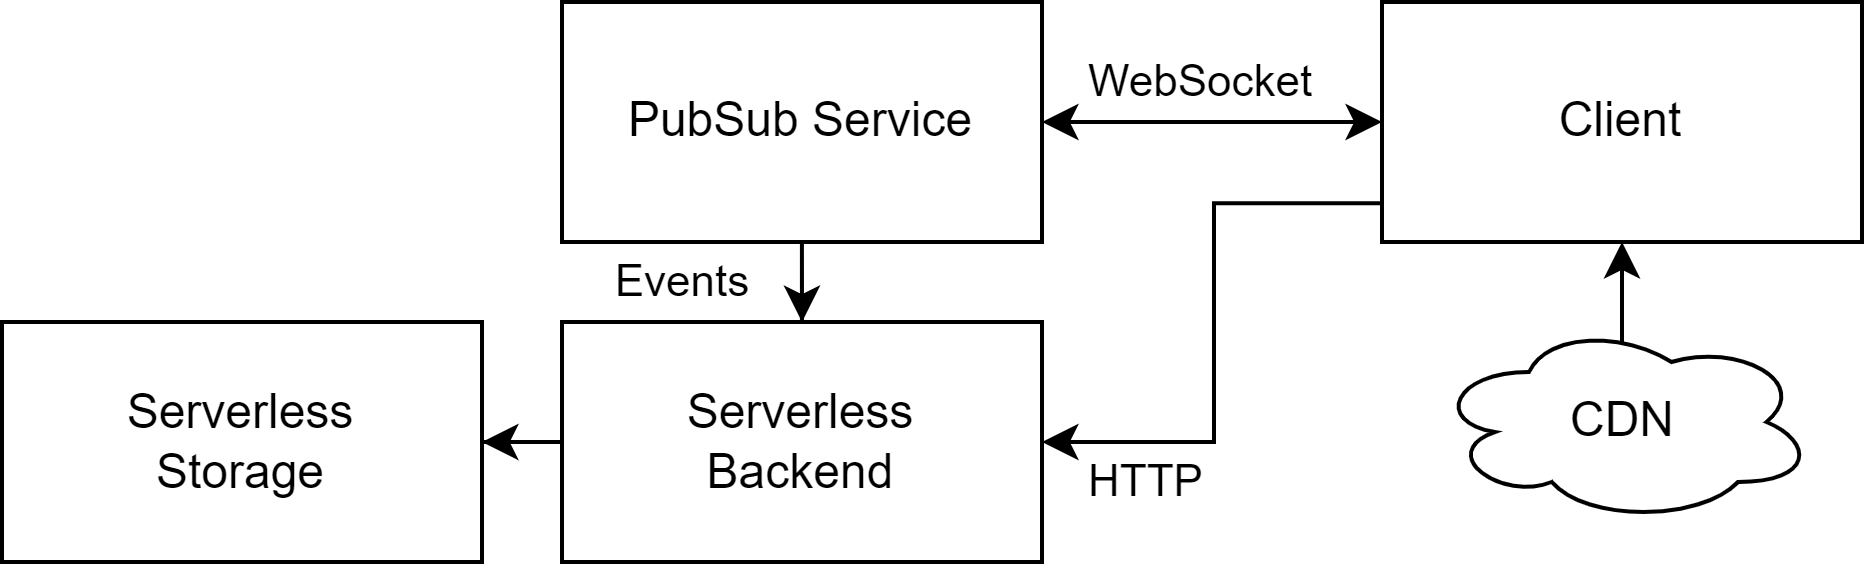
\includegraphics[width=0.7\textwidth]{architecture_services.png}
  \caption{Architecture overview}
\end{figure}

\section{Reasoning}
In this section, we explain the reasons why we chose the architecture described in the previous section for Ratable. We discuss the advantages and disadvantages of each component and how they fit our requirements and goals.

ERDTs would allow us to use peer-to-peer communication instead or in addition to client-server communication. The reason why we decided against it is that it would be out of the scope of this thesis. Implementing peer-to-peer communication would add multiple new problems in implementing communication, state management and event ordering. It is important to note that our system is very close to peer-to-peer because our server only acts as an event store and does not handle any business logic.

\subsection{Static web application}
We chose to provide our services through a web application because it allows us to reach a larger audience (e.g. mobile and desktop devices) in a more accessible way without downloads. One of our main goals was to implement our application using local-first principles. Therefore offline support as well as confidentiality and integrity of data are important to us. These concepts can be achieved using our newly proposed ERDTs. A technology that aligned very closely with our goals was Progressive Web App (PWA). So we provide PWA functionality to enable users to install Ratable as an app on their device and access it offline at any time using it like a native mobile app. We used Scala as the programming language for the web application because it has good tooling and support for web development and was a commonly used language in our research department. We did not use server-side rendering because it did not have many benefits for our use case and the tooling for Scala was not there. Instead, we used a simple and cost-effective approach of delivering the web application to users by giving access to the static files through a CDN.

\subsection{Serverless backend} 
We chose to use a serverless backend because it is very cost-effective (in fact free with our cloud provider), simple to deploy without any system configuration issues, and scalable to handle variable workloads. The main drawback of serverless is that it requires a special design for the application to work in a stateless and event-driven environment. However, this was not a major issue for us because we wanted to create a cloud-native solution and we implemented enough abstraction to be able to change the cloud provider without a complete rewrite. We used Scala as the programming language for the backend because it is compatible with the web application and it has good support for concurrency and distribution. We used an event sourcing pattern to persist the state changes as a sequence of events in the database, which enables us to make the state always accessible to users without violating local-first principles as well as being a core mechanic working with our ECRDTs.

\subsection{Serverless NoSQL database} 
We chose to use a serverless NoSQL database because it is also very cost-effective (again free with our cloud provider), easy to access through a cloud service API, and scalable to handle large amounts of data. The main advantage of NoSQL is that it allows us to use a flexible schema design that can accommodate changes in the data model without affecting the existing data. The main disadvantage of NoSQL is that it does not support complex queries or joins that are common in relational databases. However, this was not a problem for us because we did not have specific requirements for querying or joining data and we followed the recommended way by our cloud provider to use this service. The database also supports transactions and consistency guarantees for the data operations, which are important for ensuring data integrity and reliability.

\subsection{Pub-sub service}
We chose to use a pub-sub service because it enables us to provide real-time updates and asynchronous messaging between the web application and the backend. The pub-sub service manages the WebSocket connections and publishes or subscribes to messages based on events. This way, we can avoid polling or refreshing the page to get updates from the backend, which improves the user experience and reduces the network traffic. The pub-sub service also allows us to implement a publish-subscribe pattern that decouples the producers and consumers of messages, which increases the modularity and scalability of our system.

\subsection{Protobuf protocol}
We chose to use protobuf as the protocol for defining and encoding the messages between the web application and the backend because it has several advantages over JSON, which is commonly used for web applications. Protobuf supports ‘one of’ relationships, which are useful for representing different types of messages with different content. Protobuf also reduces the message size compared to JSON, which improves network performance and bandwidth usage. Protobuf also provides type safety and compatibility checks for the messages, which prevents errors and conflicts in communication~\cite{protobuf}.

\section{Project Structure}
In this section, we describe the project structure of Ratable and how it reflects the architecture and design choices we made in the previous sections. We explain how we organized the code into modules, layers, and services, and how we ensured the testability and modularity of our system.

Ratable consists of two main applications: the serverless backend and the web application. The serverless backend runs as a cloud function that accepts messages over HTTP or events over WebSockets from the web application or the pub-sub service. The web application runs as a static web page that provides an interface to the user and communicates with the backend or the pub-sub service. Additionally, we have a common core module that contains the domain model, the ERDT implementation, and all protobuf definitions that model the communication between the backend and the web application.

Both the web application and the backend are structured similarly into two main layers: the application layer and the device layer. The application layer contains the business logic and the use cases of the system. The device layer contains the interaction with the device resources, such as the network, the database, or the user interface. Between these two layers, there can be additional supportive layers that abstract away the device layer or add new functionality, such as a state layer that manages the state changes and events.

Layers interact with each other using services. Services are classes or objects that provide specific functionality or operations to other components. We use dependency injection to inject the services that each component needs. Generally, services should only request services from the same layer or a lower layer. This is to prevent cyclic dependencies and to maintain a clear separation of concerns.

The application layer is structured differently between the web application and the backend. In the web application, we use a use case-oriented approach. This means that we define different use cases that correspond to different user actions or scenarios, such as rating a Ratable. Each use case is implemented as a service that interacts with other services from the same layer or lower layers. We use a state layer to manage the state changes and events that result from executing a use case. The state layer uses ERDTs to ensure eventual consistency and conflict resolution for concurrent updates. It also interacts with the device layer to persist or synchronize the state with the backend or the pub-sub service. The device layer uses protobuf to encode or decode the messages that are sent or received over HTTP or WebSockets. It also provides an interface to access or manipulate the user interface aspects, such as routing.

In the backend, we use an event-driven approach. This means that we define different gateways that correspond to different sources or sinks of events in our system, such as HTTP requests or WebSocket connections from pub-sub messages. Each gateway is implemented as a service that interacts with other services from the same layer or lower layers. We use handlers to process and respond to the events that are received or sent by the gateways. In handling the state the handlers only persist the list of events without actually caring about the contents. The backend's only responsibility is to act as an event store. The device layer uses protobuf to encode or decode the messages that are sent or received over HTTP or WebSockets. The device layer also provides an interface to access or manipulate the database or the pub-sub service.

\section{State Managment}
In this section, we describe the state layer that we use in the web application to manage the state changes and events that result from using ERDTs. ERDTs are a core part of this thesis and they provide a new way to work with data in a distributed and eventually consistent system. We explain how we designed the state layer to provide a convenient and simple interface for the programmer to interact with ERDTs, while also abstracting away the complexity of operation-based CRDTs.

The state layer consists of two main components: repositories and aggregate views. A repository is a class that represents a collection of aggregates that share the same ERDT type. An aggregate is an instance of an ERDT that has a unique identifier and a state. The state is a result of a sequence of events that are applied to the ERDT to produce a value. The actual events are only stored in the server acting as our event store. The programmer can use the repository to create a new aggregate or load an existing one by providing its identifier. It is currently not possible to delete an aggregate from the repository.

An aggregate view is an object that represents a single aggregate and allows the programmer to listen for changes and submit events. The aggregate view is the only way to interact with aggregates outside of the state layer. The programmer can use the aggregate view to access or modify the value of the aggregate by applying events. The events are encoded using protobuf and sent to the backend or the pub-sub service using the device layer. The aggregate view also receives events from the backend or the pub-sub service and applies them to the aggregate state using the ERDT logic. The aggregate view notifies the programmer about any changes in the value of the aggregate using callbacks or observables.

\begin{lstlisting}
trait AggregateView[A, C, E <: Event[A, C]]:
  def effect(event: E, context: C)(using EffectPipeline[A, C]): EitherT[Future, RatableError, Unit]
  def listen: Signal[A]
\end{lstlisting}

Internally the aggregate is contained by an \texttt{AggregateFacade}. It contains the concrete ERDT value and allows free mutations around it. This free ability of free mutations is needed for operations like acknowledging sent events. This additional abstraction is needed because we do not store the ERDT directly. We need additional wrappers to enable communication and asynchronous mutations. 

\begin{lstlisting}
class AggregateFacade[A, C <: IdentityContext, E <: Event[A, C]](
  private val initial: EventBufferContainer[A, C, E]
):
  def listen: Signal[EventBufferContainer[A, C, E]] = variable

  def mutate(
    f: EventBufferContainer[A, C, E] => EitherT[Future, RatableError, EventBufferContainer[A, C, E]]
  ): EitherT[Future, RatableError, EventBufferContainer[A, C, E]] = ...

\end{lstlisting}

These aggregate facades are then created and cached by the \texttt{AggregateFacadeProvider} so that only one exists per aggregate at any moment. Around the \texttt{AggregateFacadeProvider} we have the \texttt{AggregateViewProvider} which converts aggregate facades into aggregate views. 

\begin{figure}[h]
  \centering
  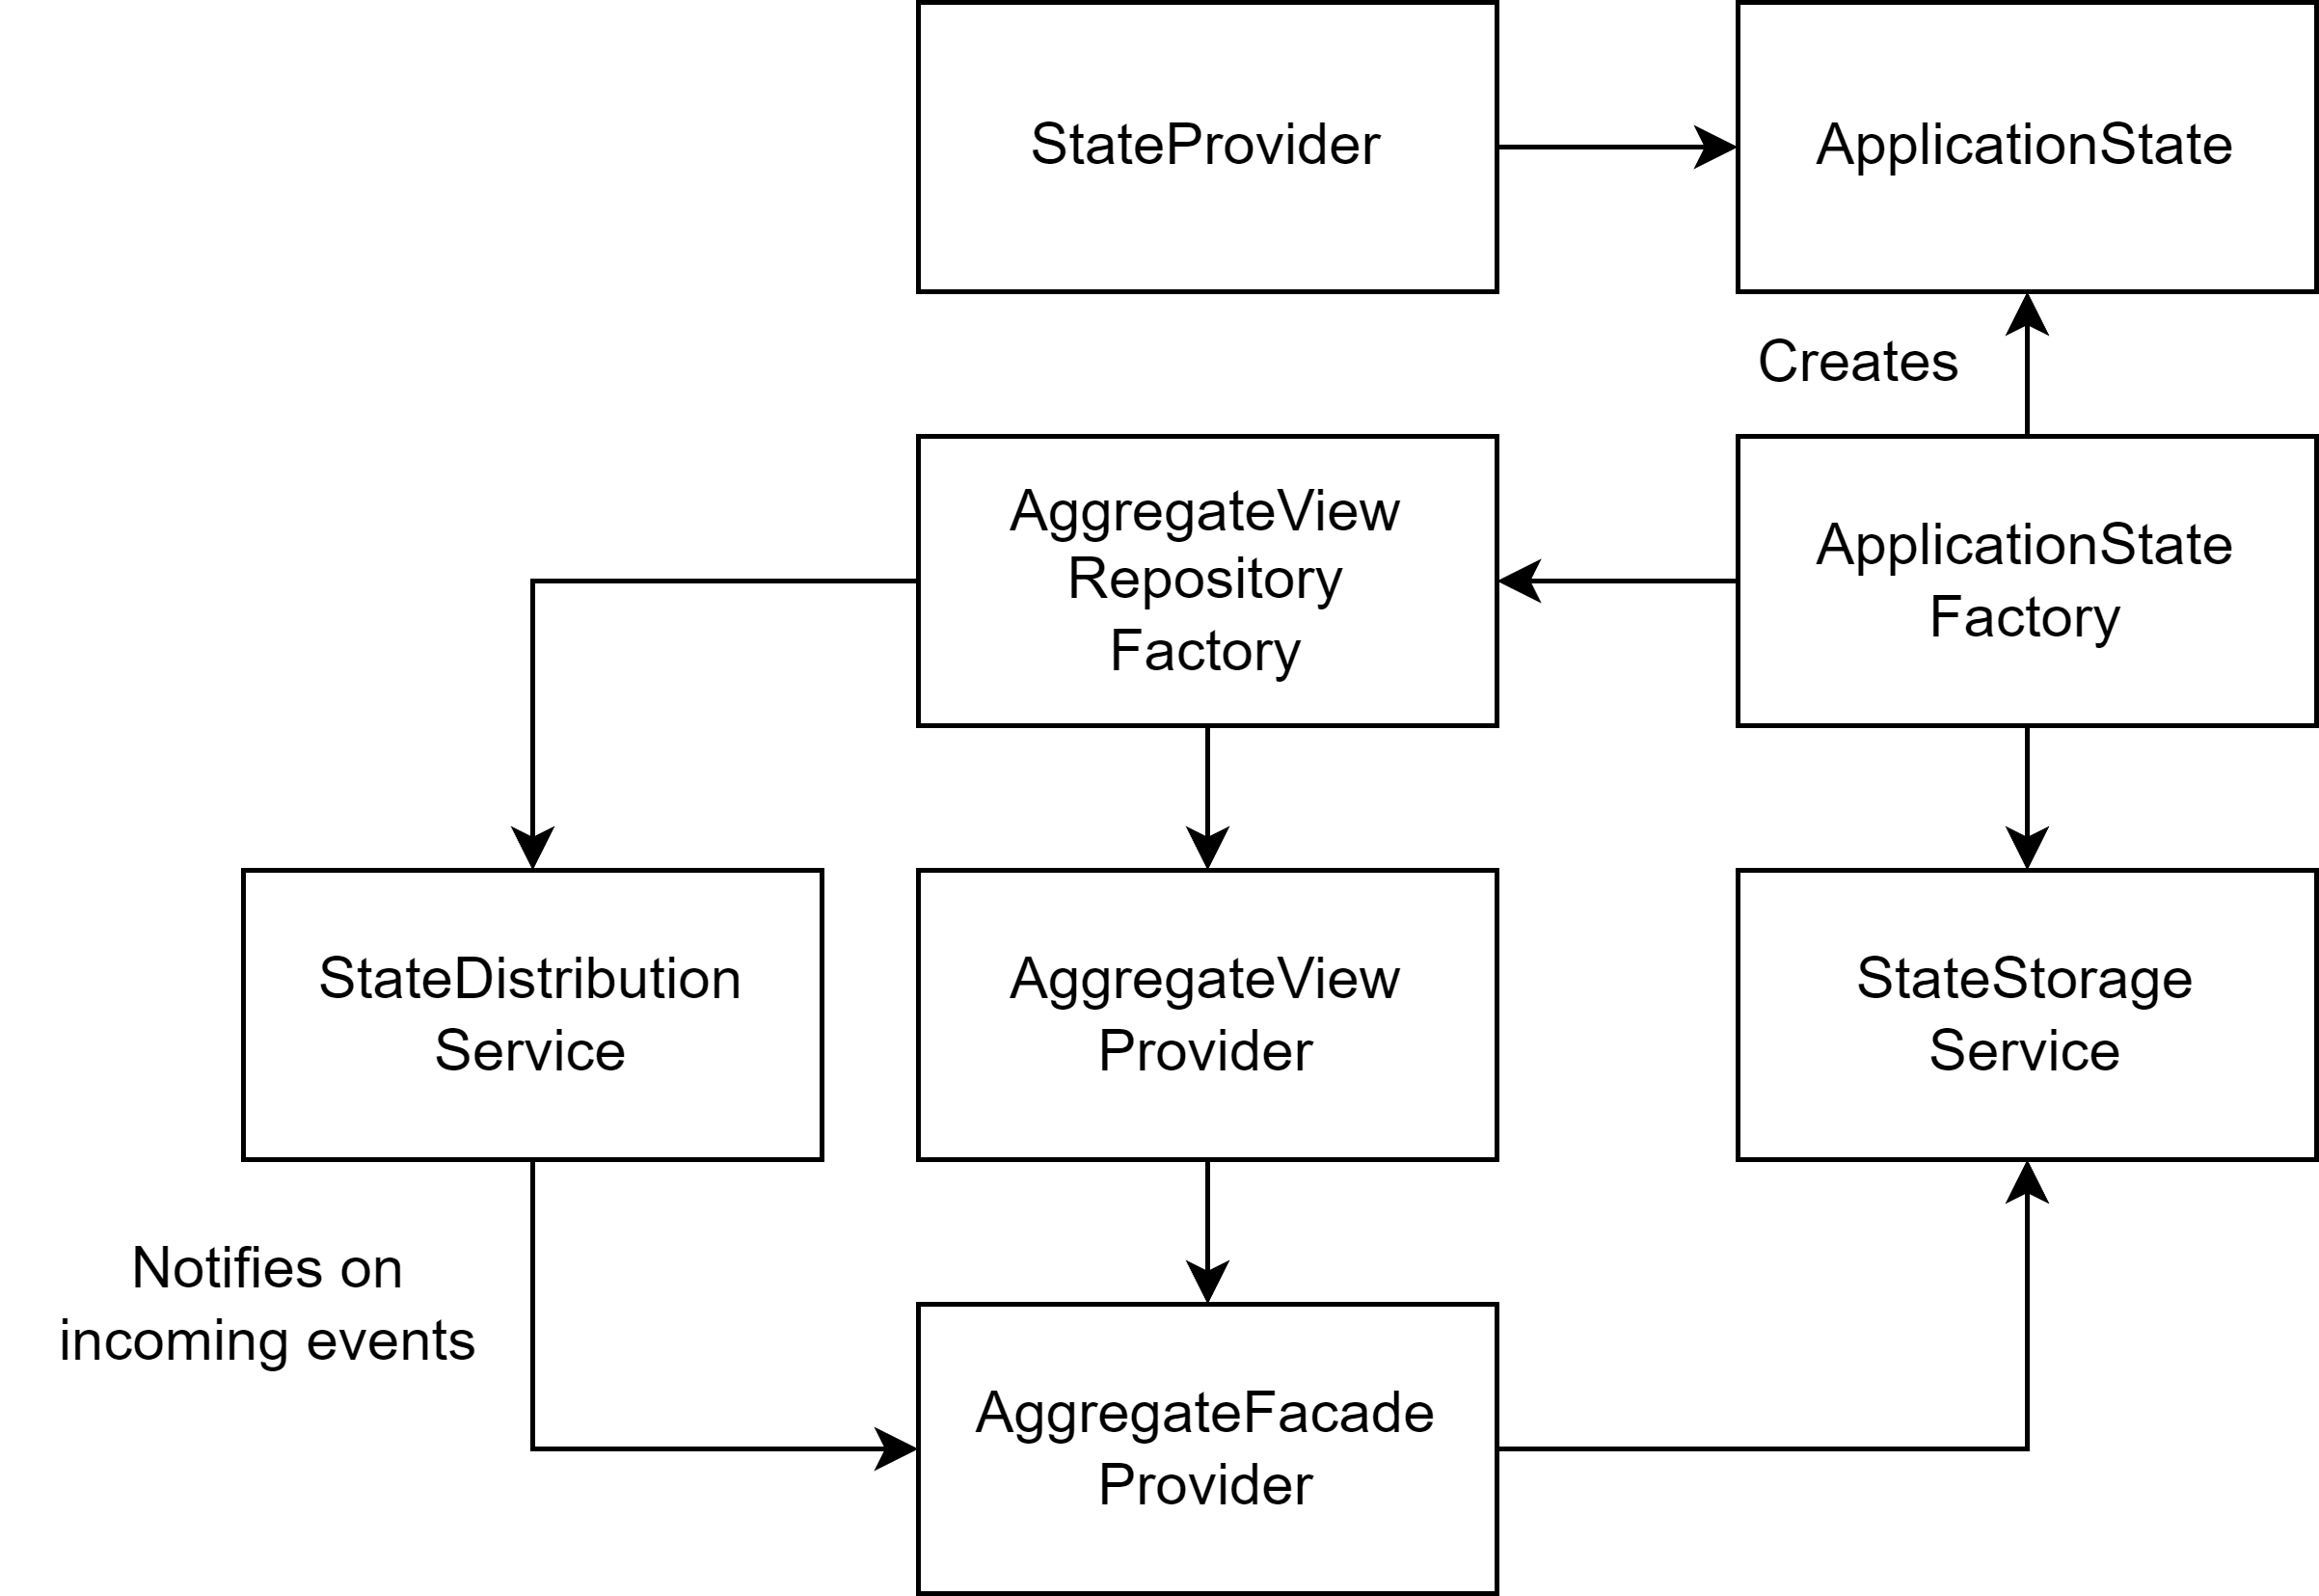
\includegraphics[width=0.7\textwidth]{state.png}
  \caption{Architecture overview}
\end{figure}

Access to the \texttt{AggregateViewProvider} is handled through \texttt{AggregateViewRepository} which is created through the \texttt{AggregateViewRepositoryFactory} and then saved as \texttt{ApplicationState}. The separation between \texttt{AggregateViewProvider} and \texttt{AggregateFacadeProvider} is needed so that other state services can access the aggregate facades instead of the aggregate views. The two services currently using this are the \texttt{StateStorageService} handling loading and saving aggregates on the user device and the \texttt{StateDistributionService} handling outgoing and incoming events. 

Using this abstraction we can now provide an \texttt{ApplicationState} like the following.

\begin{lstlisting}
case class ApplicationState(
  ratables: AggregateViewRepository[Ratable, RatableContext, RatableEvent],
  library: AggregateViewRepository[RatableLibrary, RatableLibraryContext, RatableLibraryEvent]
)
\end{lstlisting}

\chapter{Conclusion and Future Work}
In this thesis, we proposed a new variant of operation-based CRDTs to support the development of domain-independent extensions especially to solve the problem of security enabling authentication and authorization. Additionally, we developed an application called Ratable showcasing the use, the benefits as well as a possible architecture to implement modern local-first applications using ERDTs.

The here proposed solution focuses on domain problems similar to Ratable with non-frequent events describing user actions. This is especially important because CRDTs are usually often used in real-time text editing/collaboration software where frequent events are expected. Our solution would likely not be suitable for such applications because of quickly increasing storage costs and non-optimal latency because of extension pipelines.

For problem domains like Ratable it provides an elegant way to implement complex business logic in a distributed local-first and eventually consistent system. While the here proposed solution does not support peer-to-peer systems, it is possible to implement a solution that does.

\minisec{Peer to Peer}
ERDTs use the single server as an event store and as means of communication with other peers. Authentication, authorization, as well as business-logic, is handled fully by the clients themselves therefore extending the existing ERDTs to enable peer-to-peer systems is not very difficult. Two things have to be implemented and redesigned.

\begin{itemize}
  \item Every client has to act as an event store for itself as well as for other clients. This is especially important when a client wants to query new events it has not seen yet. Since the server is not available in a peer-to-peer system, this system has to implement additional redundancy to ensure data availability.
  \item The communication between clients has to be replaced by a peer-to-peer network using technologies like WebRTC. This poses new challenges like unreliable connections, high latency and the need for handshakes. Additionally usually technologies supporting peer-to-peer connections only allow a limited number of concurrent connections. In larger networks, one would have to implement a custom topology to ensure that all clients can communicate with each other.
\end{itemize}

While achieving peer-to-peer systems might be possible, it is with current peer-to-peer technologies like WebRTC rarely the best solution for applications. Data integrity and security can already be achieved by ERDTs using additional end-to-end encryption between clients. The overhead of implementation difficulty and complexity as well as limitations of peer-to-peer systems like unreliable connections and high latency make it not worth the effort. Additionally often pure peer-to-peer systems are not possible to implement because of the need for handshakes between clients before they can communicate with each other or the need for high data availability.

\minisec{ERDTs}
In the current state, ERDTs are not perfect and can be further improved. The following are some ideas for future work.

\begin{itemize}
  \item ERDTs do not support the signing of events by themselves. It has to be implemented manually by the developer. In the future, it might be possible to integrate event signing into the ERDTs themselves or even better into a custom extension.
  \item Currently we have separate concepts of events and contexts which are then associated together. It might be possible to combine these two concepts into one and then explicitly associate them together. This would make the implementation of ERDTs easier and more intuitive.
  \item Currently ERDTs do not have an event store. When extending this concept directly into peer-to-peer systems it would be beneficial to have an event store. The drawback of this is that it would decrease the flexibility of ERDTs.
\end{itemize}

Currently, ERDTs only build upon the concept of operation-based CRDTs because they support the most intuitive way of implementing authorization. However, there are use cases where state-based CRDTs are more suitable, especially in the case of frequent events. In the future, it might be possible to combine the two concepts to create a more general solution supporting both use cases. This could be done by allowing the merging of events. This would solve the problem of long term storage as well as network throughput. 

\printbibliography

\end{document}
